

%!TEX root = ../thesis.tex
%******************************************************************************
\chapter[Conceptual Framework]{A Conceptual Framework for Feedback-Controlled Bulk Data Processing Systems}\label{ch:conceptual_framework}

%******************************************************************************

\section{Introduction} 

\begin{itemize}
	\item The concept for an adaptive Middleware for bulk data processing presented in chapter \ref{ch:adaptive_middleware} describes the ``What'' (what needs to be done) but not the ``How'' (how should it be done).
	\item The design, implementation and operation of such a system differs from common approaches to implement enterprise systems (what are these differences?)
	\begin{itemize}
		\item Design: Defining Service interfaces, defining aggregation rules, defining transports, defining integration architecture
		\item Implementation: Service implementation, Service Optimisation
		\item Operation: controller tuning, monitoring
	\end{itemize}
	\item In order to guide the implementation of an adaptive system for bulk data processing, a conceptual framework is needed
	\item It defines views, roles and tasks and their dependencies to describe the necessary steps for design, implementation and operation of system describe in Chapter \ref{ch:adaptive_middleware}.
	\item It only describes concepts that are specific to the design and implementation of an Adaptive Middleware as described in the previous chapter. It does not describe common concepts for softwar development.
	\item The conceptual model can be tailored to specific projects requirements, it does not have to be followed strictly.
\end{itemize}

\begin{figure}
	[htpb] \centering 
	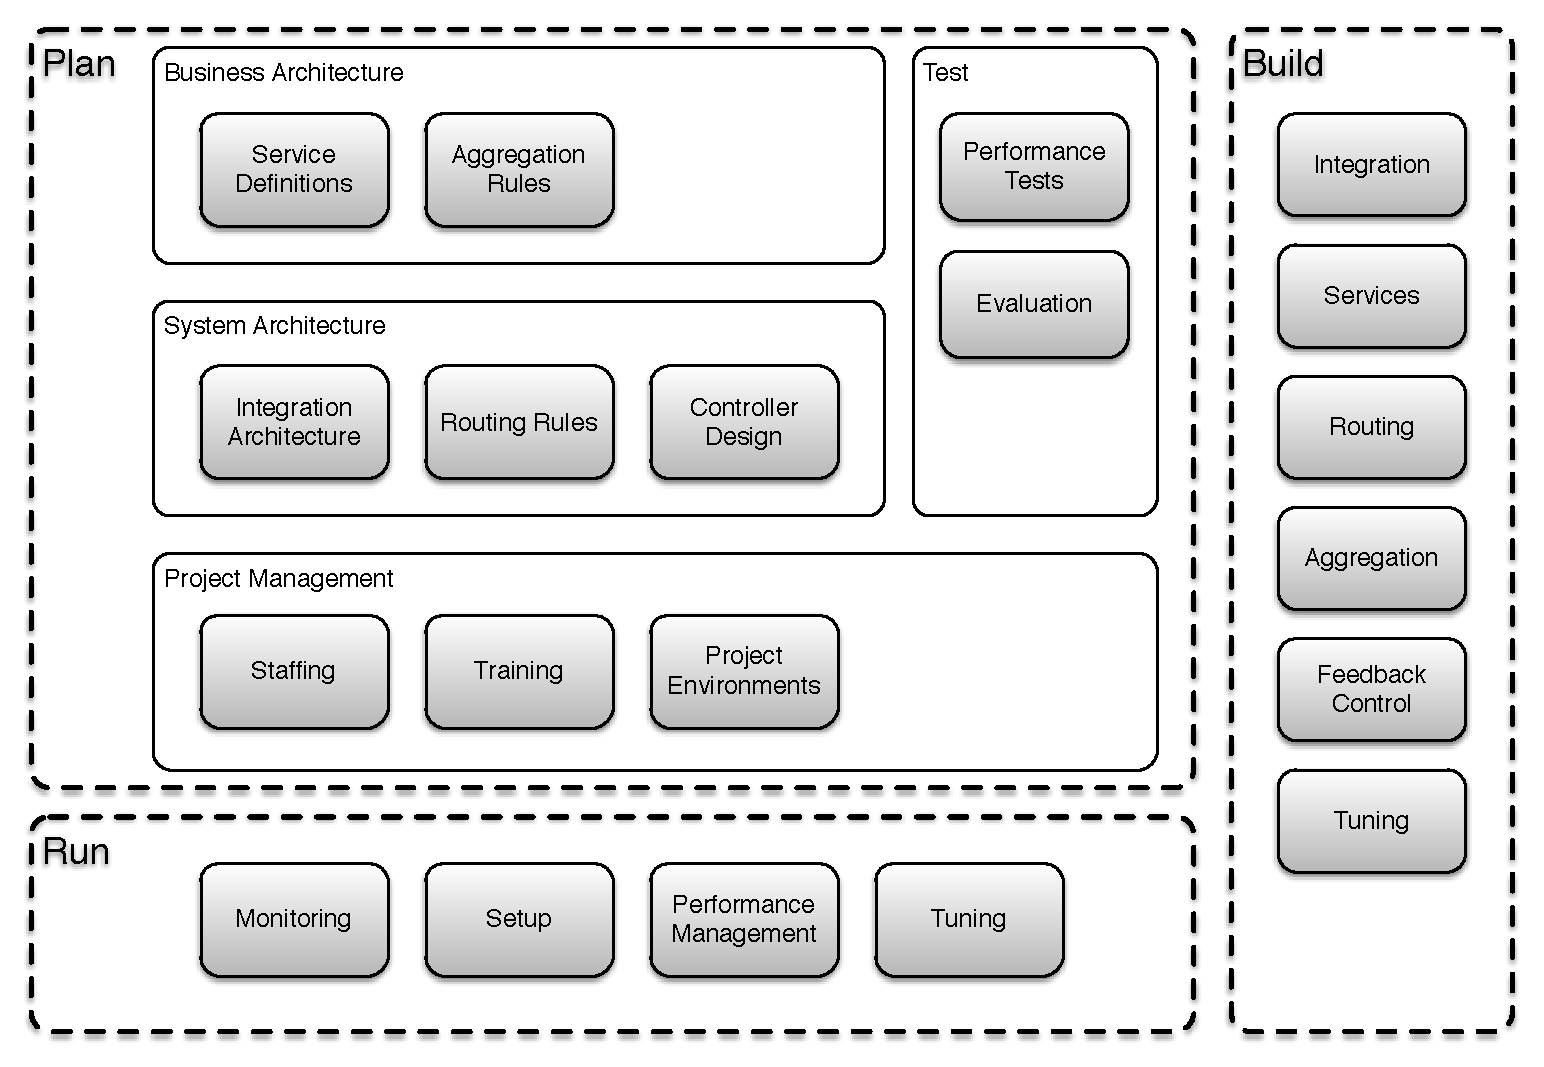
\includegraphics[width=\textwidth]{ch6_overview} \caption{Overview of Conceptual Framework} \label{fig:ch6_overview} 
\end{figure}

\section{Metamodel} 
The conceptual framework consists of the following entities:
\begin{itemize}
	\item Phase
	\begin{itemize}
		\item contains Tasks
	\end{itemize}
	\item Role
	\begin{itemize}
		\item processes Tasks
	\end{itemize}
	\item Task
	\begin{itemize}
		\item is contained in a Phase
		\item is processed by a Role
		\item produces Artifacts
		\item uses Tools
	\end{itemize}
	\item Deliverable
	\begin{itemize}
		\item is produced by a Task
	\end{itemize}
	\item Tool
	\begin{itemize}
		\item is used by a Task
	\end{itemize}
\end{itemize}

\begin{figure}
	[htpb] \centering 
	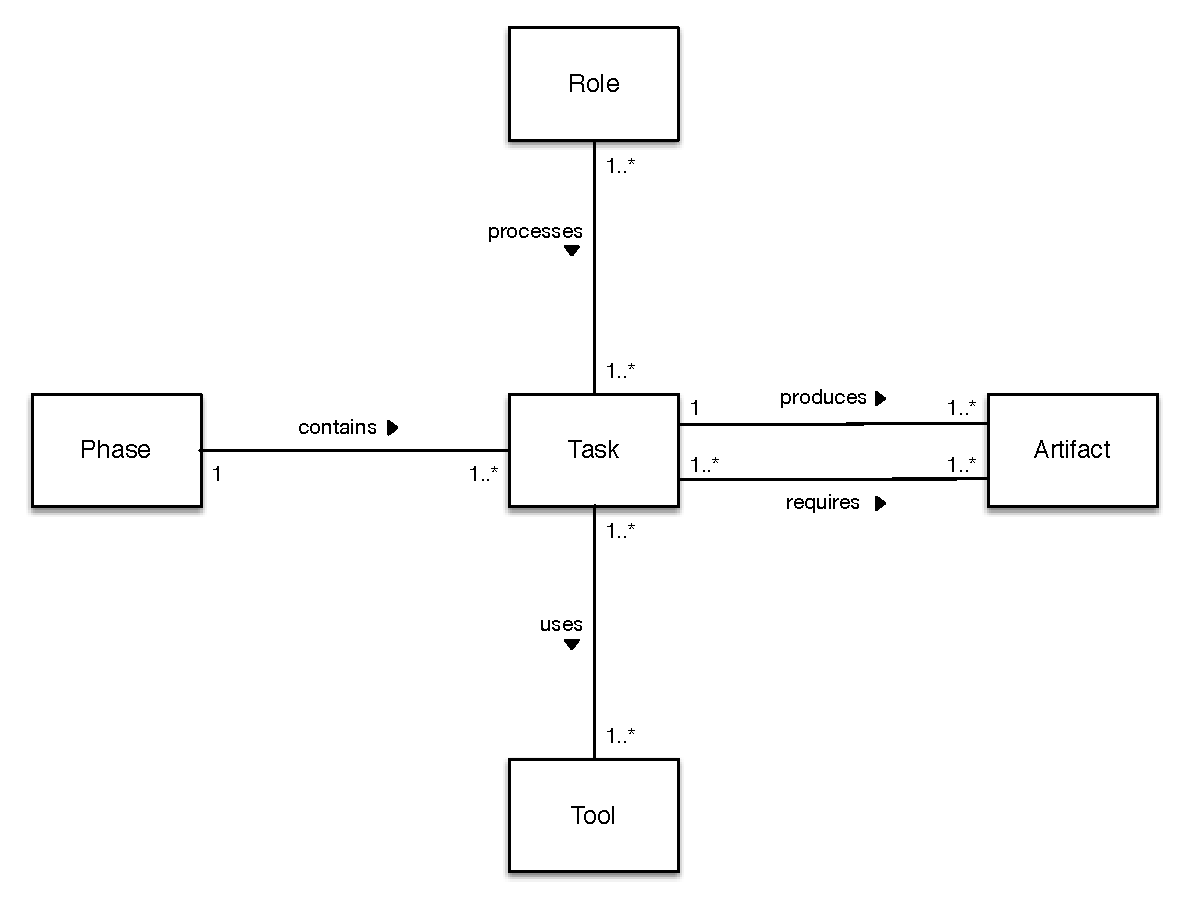
\includegraphics[width=\textwidth]{ch6_metamodel} 
	\caption{Metamodel} 
	\label{fig:ch6_metamodel} 
\end{figure}

\section{Phase}

\begin{itemize}
	\item Phases are the toplevel building blocks
	\item The framework defines the following phases
	\begin{itemize}
		\item Plan
		\item Build
		\item Run
	\end{itemize}
	\item Phases are aligned to phases commonly used by other software development frameworks and methodologies (examples?)
	\item It should be noted that the framework defines no requirements regarding the general order or mode in which theses phases should be processed. It is therefore possible to use this framework with different software development methodologies such as the Waterfall model, Scrum or the V-Modell.
\end{itemize}

\subsection{Plan}
\begin{minipage}{\textwidth}
	\captionof{table}{Phase: Plan}\label{table:ch6_View_Plan}
	\begin{tabular}
		{|m{2cm}|m{10cm}|} \hline \bfseries Phase & Plan\\
		\hline \bfseries Description & This phase contains tasks concerning the technical and business design of the system.\\
		\hline \bfseries Tasks & 
		\begin{itemize}
			\item Define Service Interfaces
			\item Define Aggregation Rules
			\item Define Integration Architecture
			\item Define Routing Rules
			\item Define Controller Architecture
			\item Define Performance Tests
			\item Evaluate Test Results
			\item Perform Staffing
			\item Define Training Concept
			\item Source Projct Environments
		\end{itemize}
		\\
		\hline \bfseries Roles &
		\begin{itemize}
			\item Project Manager
			\item Business Analyst
			\item System Architect
			\item Test Engineer
		\end{itemize}
		\\
		\hline 
	\end{tabular}
\end{minipage}

\subsection{Build}
\begin{minipage}{\textwidth}
\captionof{table}{Phase: Build}\label{table:ch6_View_Build}
\begin{tabular}
	{|m{2cm}|m{10cm}|} \hline \bfseries Phase & Build\\
	\hline \bfseries Description & This phase contains tasks concerning the implementation of the system.\\
	\hline \bfseries Tasks & 
	\begin{itemize}
		\item Implement Integration Architecture
		\item Implement Service Interfaces
		\item Implement Aggregation Rules
		\item Implement Routing Rules
		\item Implement Feedback-Control	
		\item Perform Controller Tuning
	\end{itemize}
	\\
	\hline \bfseries Roles &
	\begin{itemize}
		\item Software Engineer
	\end{itemize}
	\\
	\hline 
\end{tabular}
\end{minipage}

\subsection{Run}
\begin{minipage}{\textwidth}
\captionof{table}{Phase: Run}\label{table:ch6_View_Run}
\begin{tabular}
	{|m{2cm}|m{10cm}|} \hline \bfseries Phase & Run\\
	\hline \bfseries Description & This phase contains tasks concerning the operation of the implemented system in the production environment. \\
	\hline \bfseries Tasks & 
	\begin{itemize}
		\item Setup Monitoring Infrastructure
		\item Setup Test Environment
		\item Perform Performance Tests
	\end{itemize}
	\\
	\hline \bfseries Roles &
	\begin{itemize}
		\item Operations Engineer
		\item Test Engineer
	\end{itemize}
	\\
	\hline 
\end{tabular}
\end{minipage}

\section{Roles} 

\begin{itemize}
	\item Roles describe responsibilities and skills
	\item Describe who does something
	\item A Task is processed by a role
	\item Roles are not the same as persons, a person can fulfill multiple roles at the same time
\end{itemize}

The Conceptual Framework defines the following Roles:
\begin{itemize}
	\item Business Architect
	\item System Architect 
	\item Software Engineer
	\item Test Engineer
	\item Operations Engineer
	\item Project Manager
\end{itemize}

\subsection{Business Analyst}
\begin{minipage}{\textwidth}
\captionof{table}{Business Architect} \label{table:ch6_Role_Business_Analysist}
\begin{tabular}
	{|m{2cm}|m{10cm}|} \hline \bfseries Role & Business Analyst\\
	\hline \bfseries Description & The Business Architect is responsible for designing the business architecture of the system, including the definition of services and aggregation rules.\\
	\hline \bfseries Tasks & 
	\begin{itemize}
		\item Define Service Interfaces
		\item Define Aggregation Rules
	\end{itemize}
	\\
	\hline 
	\bfseries Needed skills &
	\begin{itemize}
		\item Integration styles and patterns, e.g. \ac{SOA}
		\item Concepts of the Adaptive Middleware for Bulk Data Processing
		\item Business domain knowledge
	\end{itemize}
	\\
	\hline
\end{tabular}
\end{minipage}

\subsection{System Architect} 
\begin{minipage}{\textwidth}
\captionof{table}{System Architect}\label{table:ch6_Role_System_Architect}
\begin{tabular}
	{|m{2cm}|m{10cm}|} \hline \bfseries Role & System Architect\\
	\hline \bfseries Description & The System Architect is responsible for designing the technical architecture of the system, including the integration and controller architecture.\\
	\hline \bfseries Tasks & 
	\begin{itemize}
		\item Define Integration Architecture
		\item Define Controller Architecture
	\end{itemize}
	\\
	\hline
	\bfseries Needed skills & 
	\begin{itemize}
		\item System modelling languages, e.g. \ac{UML} and tools
		\item Integration styles and patterns, e.g. \ac{SOA}
		\item Processing styles, e.g. batch and single-event processing
		\item Integration middleware technologies and products, e.g. Apache Camel, \ac{ESB}
		\item Concepts of the Adaptive Middleware for Bulk Data Processing
		\item Control theory
	\end{itemize}
	\\
	\hline
\end{tabular}
\end{minipage}

\subsection{Software Engineer}
\begin{minipage}{\textwidth}
\captionof{table}{Software Engineer} \label{table:ch6_Role_Developer}
\begin{tabular}
	{|m{2cm}|m{10cm}|} \hline \bfseries Role & Developer\\
	\hline \bfseries Description & The Developer is responsible for the implementation of the system, including the implementation and tuning of the feeback-controll loop.\\
	\hline \bfseries Tasks & 
	\begin{itemize}
		\item Implement Integration Architecture
		\item Implement Service Interfaces
		\item Implement Aggregation Rules
		\item Implement Routing Rules
		\item Implement Feedback-Control
		\item Perform Controller Tuning
	\end{itemize}
	\\
	\hline 
	\bfseries Needed skills &
	\begin{itemize}
		\item Integration styles and patterns, e.g. \ac{SOA}
		\item Processing styles, e.g. batch and single-event processing
		\item Batch optimisations
		\item Integration middleware technologies and products, e.g. Apache Camel, \ac{ESB}
		\item Concepts of the Adaptive Middleware for Bulk Data Processing
		\item Control theory
	\end{itemize}
	\\
	\hline
\end{tabular}
\end{minipage}

\subsection{Test Engineer}
\begin{minipage}{\textwidth}
\captionof{table}{Tester} \label{table:ch6_Role_Tester}
\begin{tabular}
	{|m{2cm}|m{10cm}|} \hline \bfseries Role & Test Engineer\\
	\hline \bfseries Description & The Tester is responsible for defining and performing the performance tests of the system.\\
	\hline \bfseries Tasks & 
	\begin{itemize}
		\item Define Performance Tests
		\item Perform Performance Tests
		\item Evaluate Performance Tests
	\end{itemize}
	\\
	\hline
	\bfseries Needed skills &
	\begin{itemize}
		\item Design and evaluation of performance tests
		\item Concepts of the Adaptive Middleware for Bulk Data Processing
		\item Control theory (basics)
	\end{itemize}
	\\
	\hline
\end{tabular}
\end{minipage}

\subsection{Operations Engineer}
\begin{minipage}{\textwidth}
\captionof{table}{Operations Engineer} \label{table:ch6_Role_Operations_Engineer}
\begin{tabular}
	{|m{2cm}|m{10cm}|} \hline \bfseries Role & Operations Engineer\\
	\hline \bfseries Description & The Operations Engineer is responsible for operating the system, including setup, deployment and monitoring.\\
	\hline \bfseries Tasks & 
	\begin{itemize}
		\item Setup Monitoring Infrastructure
		\item Setup System Environments
		\item Perform System Tuning
	\end{itemize}
	\\
	\hline
	\bfseries Needed skills &
	\begin{itemize}
		\item Monitoring technologies and products, e.g. \ac{JMX}
		\item Concepts of the Adaptive Middleware for Bulk Data Processing
	\end{itemize}
	\\
	\hline
\end{tabular}
\end{minipage}

\subsection{Project Manager}
\begin{minipage}{\textwidth}
\captionof{table}{Project Manager} \label{table:ch6_Role_Project_Manager}
\begin{tabular}
	{|m{2cm}|m{10cm}|} \hline \bfseries Role & Project Manager\\
	\hline \bfseries Description & The Project Manager is responsible for the project coordination, including the staffing and planing of the required environments.\\
	\hline \bfseries Tasks & 
	\begin{itemize}
		\item Perform Staffing
		\item Define Training Concept
		\item Source Project Environments
	\end{itemize}
	\\
	\hline 
	\bfseries Needed skills &
	\begin{itemize}
		\item Framework for Feedback-Controlled Bulk Data Processing Systems
		\item Concepts of the Adaptive Middleware for Bulk Data Processing
	\end{itemize}
	\\
	\hline
\end{tabular}
\end{minipage}

\section{Tasks}
\label{sec:ch6_tasks}

\begin{itemize}
	\item Main entities of the conceptual framework, define what should be done.
	\item Tasks depend on each other, some tasks must be processed in a certain order
	\item The Conceptual Framework only describes tasks that are specific to the design and implementation of an Adaptive Middleware for Bulk Data Processing as described in chapter \ref{ch:adaptive_middleware}. It does not describe common tasks that are needed for every software system.
	\item Figure \ref{fig:ch6_overview_tasks} shows an overview of the tasks assigned to the different phases of the Conceptual Framework.
\end{itemize}

\begin{figure}[htpb] \centering 
	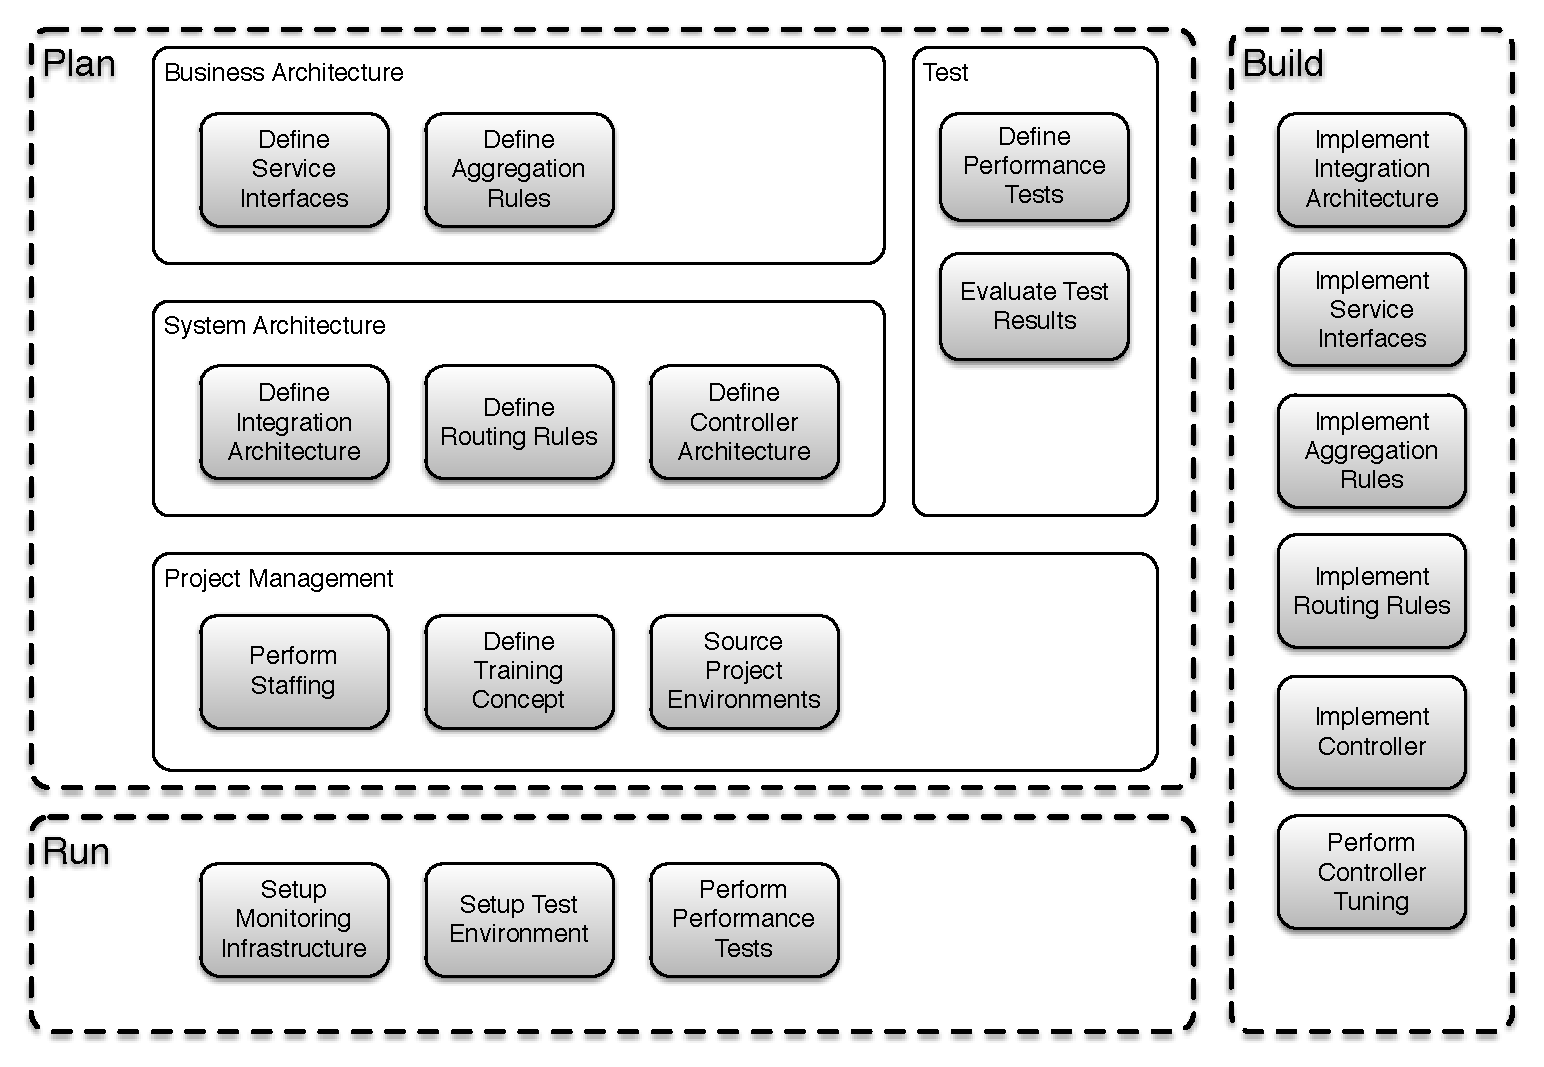
\includegraphics[width=\textwidth]{ch6_overview_tasks} 
	\caption{Overview of tasks} 
	\label{fig:ch6_overview_tasks} 
\end{figure}

\begin{itemize}
	\item Define Business Architecture
	\begin{itemize}
		\item Define Service Interfaces
		\item Define Aggregation Rules
	\end{itemize}
	\item Define System Architecture 
	\begin{itemize}
		\item Define Integration Architecture
		\begin{itemize}
			\item Transports
			\item Distribution
		\end{itemize}
		\item Define Routing Rules
		\item Define Controller Architecture 
		\begin{itemize}
			\item Define Control Problem 
			\item Define Input/Output Variables 
		\end{itemize}
		\item Define Routing Rules
	\end{itemize}
	\item Implement Controller / Feedback Loop
	\item Perform Controller Tuning 
	\begin{itemize}
		\item System Model/System Identification 
		\item Static Tests
		\item Step Tests
	\end{itemize}
	\item Implement Integration Architecture
	\item Implement Service Interfaces
	\item Implement Aggregation Rules 
	\item Implement Routing Rules
	\item Define Performance Tests 
	\item Setup Monitoring infrastructure
	\item Setup Test and Integration Environment
	\item Perform Performance Tests
	\item Evaluate Performance Test Results
	\item Define Training Concept
	\item Staffing
\end{itemize}

\subsection{Business Architecture}

\begin{itemize}
	\item The business architecture defines the business components of the system and their relationships independantly of the technical implementation.
	\item Except from the described subtasks, the task is not specific to the conceptual model.
\end{itemize}

\begin{figure}[htpb] \centering 
	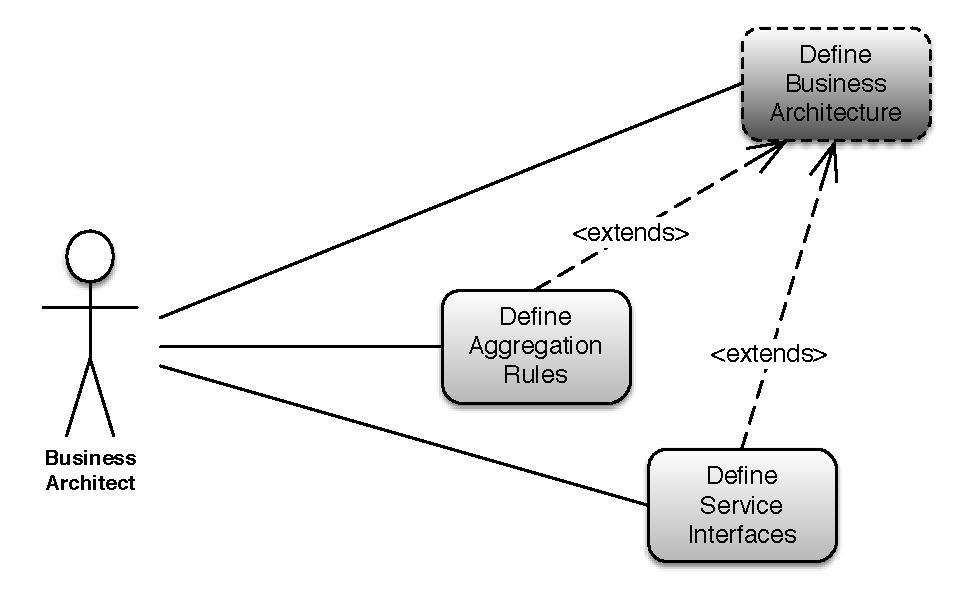
\includegraphics[width=\textwidth]{ch6_tasks_business_architecture} 
	\caption{Tasks extending the definition of the business architecture} 
	\label{fig:ch6_tasks_business_architecture} 
\end{figure}

\subsubsection{Define Service Interfaces}
\begin{minipage}{\textwidth}
\captionof{table}{Define Service Interfaces} \label{table:ch6_Task_Define_Service_Interfaces}
\begin{tabular}
	{|m{3cm}|m{10cm}|} \hline \bfseries Task & Define Service Interfaces\\
	\hline \bfseries What & 
	\begin{itemize}
		\item Structuring the functionality of the system into business services
		\item Services may already exist or need to be implemented.
		\item Definition of needed services and their operations, every service needs operations for single event and batch processing
		\begin{itemize}
			\item Distinct operations for batch and single event processing
			\item common operation for both processing styles (list interface)
		\end{itemize}
		\item Defines the structure of input and output data
		\item Does not include informations about the technical format, such as \ac{XML} or \ac{JSON}, and the integration style, such SOAP or \ac{REST}
	\end{itemize}
	\\
	\hline \bfseries Why &
	\begin{itemize}
		\item Defines the business components (services) of the system
		\item Basis for the definition of the integration architecture and the implementation of the services.
	\end{itemize}\\
	\hline \bfseries Who & Business Architect\\
	\hline \bfseries Artifacts & Service Interface Definitions\\
	\hline \bfseries Challenges & 
	\begin{itemize}
		\item Finding the appropriate services and service granularity
	\end{itemize}\\
	\hline 
\end{tabular}
\end{minipage}

\subsubsection{Define Aggregation Rules}
\begin{minipage}{\textwidth}
\captionof{table}{Define Aggregation Rules} \label{table:ch6_Task_Define_Aggregation_Rules}
\begin{tabular}
	{|m{3cm}|m{10cm}|} \hline \bfseries Task & Define Aggregation Rules\\
	\hline \bfseries What & 
	\begin{itemize}
		\item Definition of rules used in the aggregator for correlating events
		\item Different options
		\begin{itemize}
			\item No correlation
			\begin{itemize}
				\item Simple solution
				\item even distribution of events
				\item optimization is not or hardly possible
			\end{itemize}
			\item Business correlation
			\begin{itemize}
				\item analysation of processed data needed
				\item no even distribution of data (depending on correlation rule), leads to uneven distribution of latency
				\item optimization is possible
			\end{itemize}
			\item Technical correlation
			\begin{itemize}
				\item analysation of processed data needed
				\item Rules can be defined after integration architecture
				\item no even distribution of data (depending on correlation rule), leads to uneven distribution of latency
				\item optimization (?)
			\end{itemize}
		\end{itemize}
	\end{itemize}
	\\
	\hline \bfseries Why & The aggregation Rules are needed by the Aggregator to correlate events.\\
	\hline \bfseries Who & 
	\begin{itemize}
		\item Business Architect
		\item System Architect
	\end{itemize}
	\\
	\hline \bfseries Artifacts & Aggregation Rules\\
	\hline \bfseries Challenges & 
	\begin{itemize}
		\item Finding aggregation rules that allows for an even distribution of events.
		\item Technical Aggregation Rules can be defined only after the definition of the integration architecture
	\end{itemize}\\
	\hline 
\end{tabular}
\end{minipage}

\subsection{System Architecture }

\begin{figure}[htpb] \centering 
	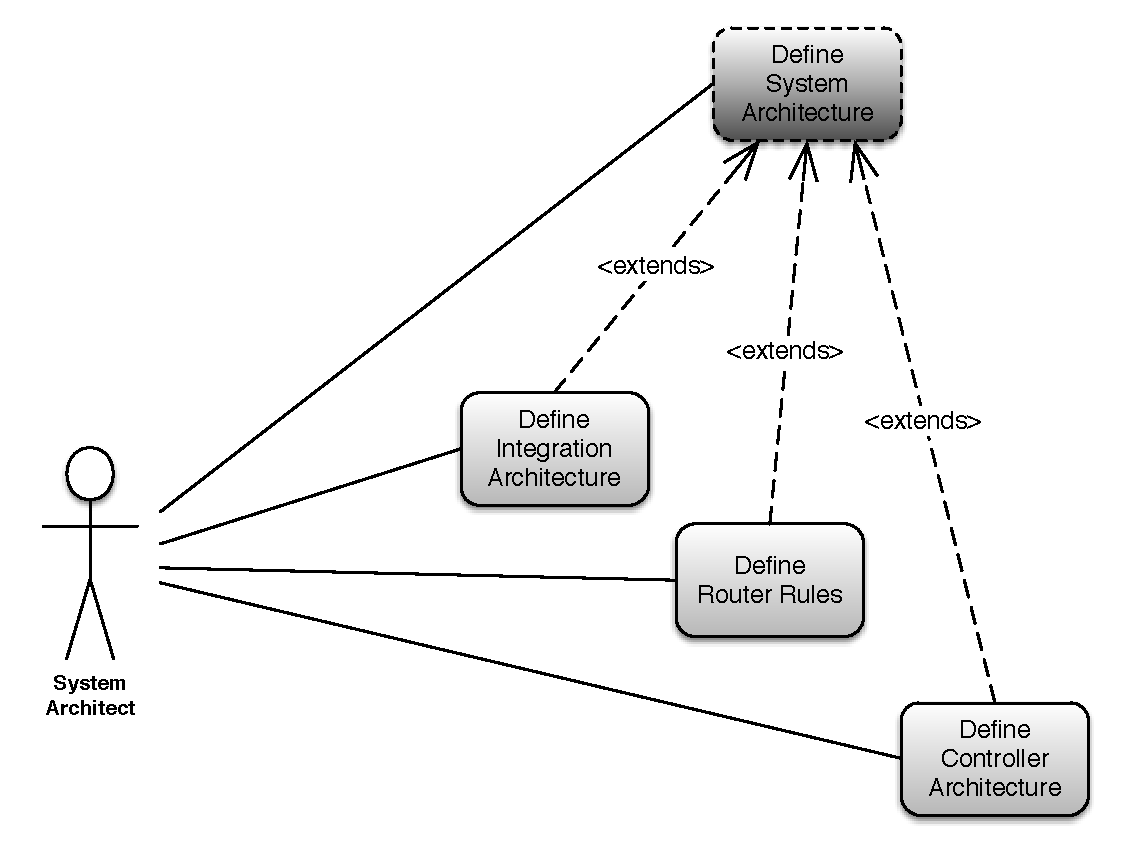
\includegraphics[width=\textwidth]{ch6_tasks_system_architecture} 
	\caption{Tasks extending the definition of the system architecture} 
	\label{fig:ch6_tasks_system_architecture} 
\end{figure}

\begin{itemize}
	\item Except from the described subtasks, the task is not specific to the conceptual model.
\end{itemize}

\subsubsection{Define Integration Architecture}
\begin{minipage}{\textwidth}
\captionof{table}{Define Integration Architecture} \label{table:ch6_Task_Define_Integration_Architecture}
\begin{tabular}
	{|m{3cm}|m{10cm}|} \hline \bfseries Task & Define Integration Architecture\\
	\hline \bfseries What &
	\begin{itemize}
		\item Definition of integration architecture
		\begin{itemize}
			\item Sychronous, e.g. webservices
			\item Asynchronous, e.g. message queues
		\end{itemize}
		\item Choosing a middleware technology or product
		\item Definition of transports
		\begin{itemize}
			\item JMS
			\item SOAP
			\item REST
			\item FTP
			\item DB
		\end{itemize}
		\item Different transports / integration patterns needed for different aggregation sizes:
		\begin{itemize}
			\item Large messages should not be transferred over the messaging bus
			\item Options for large messages:
			\begin{itemize}
				\item File-based integration and transfer using FTP or database
				\item Message-Slip EIP pattern
			\end{itemize}
		\end{itemize}
	\end{itemize}
	\\
	\hline \bfseries Why & The integration architecture defines the technologies to integrate the services into the system.\\
	\hline \bfseries Who & System Architect\\
	\hline \bfseries Input & Service Interface Definitions
	\\
	\hline \bfseries Output & Integration Architecture\\
	\hline \bfseries Challenges & Choosing the appropriate middleware technology and or product.\\
	\hline 
\end{tabular}
\end{minipage}

\subsubsection{Define Routing Rules}
\begin{minipage}{\textwidth}
\captionof{table}{Define Routing Rules} \label{table:ch6_Task_Define_Routing_Rules}
\begin{tabular}
	{|m{3cm}|m{10cm}|} \hline \bfseries Task & Define Routing Rules\\
	\hline \bfseries What & 
	\begin{itemize}
		\item Depending on the size of the aggregated message, the Router routes the message to the appropriate service endpoint, which is either optimized for batch or single event processing.
		\item The routing rules define, which service endpoint should be called for a given aggregation size.
	\end{itemize}
	\\
	\hline \bfseries Why & The routing rules define, which service endpoint should be called for a given aggregation size.\\
	\hline \bfseries Who & System Architect\\
	\hline \bfseries Input & 
		\begin{itemize}
			\item Integration Architecture
		\end{itemize}
	\\
	\hline \bfseries Output & Routing Rules Definition\\
	\hline \bfseries Challenges & Finding the data aggregation threshold to route messages to the appropriate service endpoint.\\
	\hline 
\end{tabular}
\end{minipage}

\subsection{Feedback-Control}

\begin{figure}[htpb] \centering 
	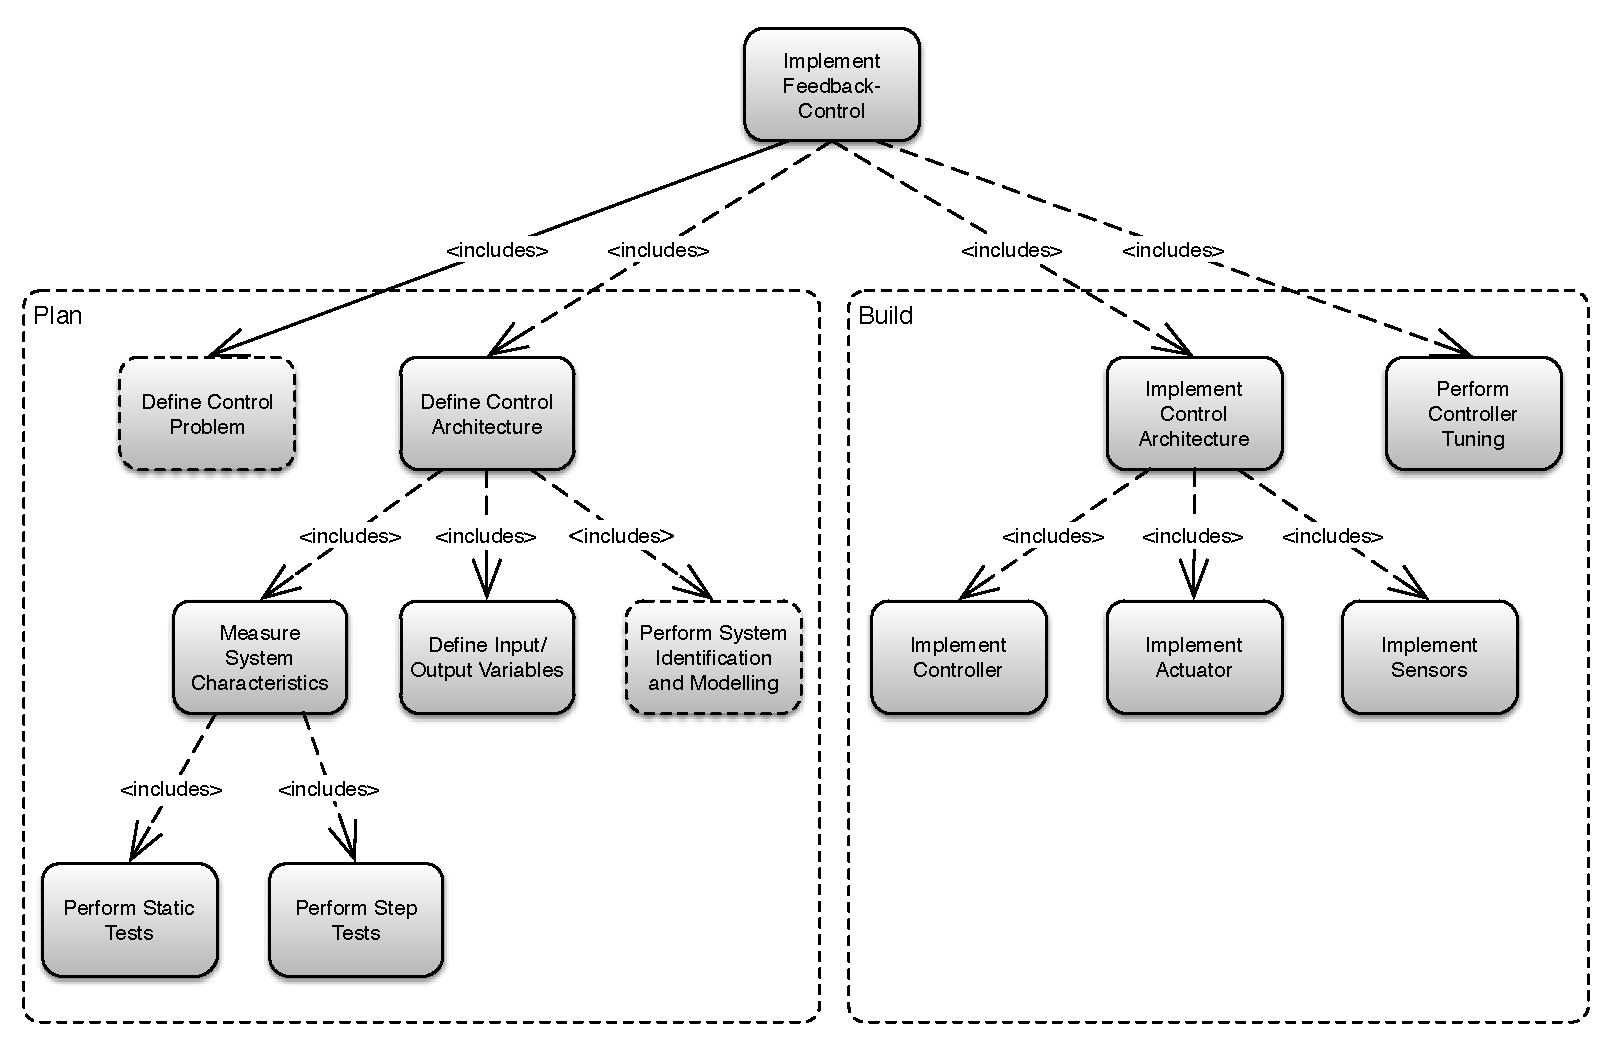
\includegraphics[width=\textwidth]{ch6_tasks_feedback_control} 
	\caption{Tasks for implementing the feedback-control loop} 
	\label{fig:ch6_tasks_feedback_control} 
\end{figure}

\begin{minipage}{\textwidth}
\captionof{table}{Define Controller Architecture} \label{table:ch6_Task_Define_Controller_Architecture}
\begin{tabular}
	{|m{3cm}|m{10cm}|} \hline \bfseries Task & Define Controller Architecture\\
	\hline \bfseries What & 
	\begin{itemize}
		\item Design of the controller architecture implemented by the system
		\item For example
		\begin{itemize}
			\item PID Controller
			\item Fuzzy Controller
		\end{itemize}
		\item Depends on control problem and system dynamics (linear, non-linear)
	\end{itemize}
	\\
	\hline \bfseries Why & The Controller Architecture is the basis for the implementation of the feedback-control loop.\\
	\hline \bfseries Who & System Architect\\
	\hline \bfseries Input & Integration Architecture\\
	\hline \bfseries Output & Controller Architecture\\
	\hline \bfseries Challenges & \\
	\hline 
\end{tabular}
\end{minipage}

\subsubsection{Define Control Problem}
\begin{minipage}{\textwidth}
\captionof{table}{Define Control Problem} \label{table:ch6_Task_Define_Control_Problem}
\begin{tabular}
	{|m{3cm}|m{10cm}|} \hline \bfseries Task & Define Control Problem\\
	\hline \bfseries What & 
	\begin{itemize}
		\item Define what properties of the system should be controlled.
		\item In case of the Adaptive Middleware (see Chapter \ref{ch:adaptive_middleware}) the control problem is already defined.
	\end{itemize}
	\\
	\hline \bfseries Why & The control problem defines the goal of the feedback-control.\\
	\hline \bfseries Who & System Architect\\
	\hline \bfseries Artifacts & Control Problem\\
	\hline \bfseries Challenges & Lorem Ipsum\\
	\hline \bfseries Best practises & Lorem ipsum\\
	\hline 
\end{tabular}
\end{minipage}

\subsubsection{Define Input/Output Variables}
\begin{minipage}{\textwidth}
\captionof{table}{Define Input/Output Variables} \label{table:ch6_Task_Define_Controller_Variables}
\begin{tabular}
	{|m{3cm}|m{10cm}|} \hline \bfseries Task & Define Input/Output Variables\\
	\hline \bfseries What &
	\begin{itemize}
		\item Definition of input and output variables of the controller
		\item for example
		\begin{itemize}
			\item Number of messages in the system
			\item Input queue length
			\item current end-to-end latency
			\item current throughput
		\end{itemize}
	\end{itemize}
	\\
	\hline \bfseries Why & The input/output variables are needed for the implementation of the controller.\\
	\hline \bfseries Who & System Architect\\
	\hline \bfseries Input & Control Problem\\
	\hline \bfseries Output & Input/Output Variables\\
	\hline \bfseries Challenges & The selected input variables should be measured easily and directly, without delay such as when calculating averages.\\
	\hline 
\end{tabular}
\end{minipage}

\subsubsection{Implement Controller}
\begin{minipage}{\textwidth}
\captionof{table}{Implement Controller / Feedback Loop} \label{table:ch6_Task_Implement_Controller}
\begin{tabular}
	{|m{3cm}|m{10cm}|} \hline \bfseries Task & Implement Feedback-Control Loop\\
	\hline \bfseries What & 
	\begin{itemize}
		\item Implementation of Controller Architecture including
		\begin{itemize}
			\item Sensors
			\item Controller
			\item Actuator
		\end{itemize}
		\item Implement JMX Beans for monitoring purposes
		\item Implement mechanisms for performing static and step tests.
	\end{itemize}
	\\
	\hline \bfseries Why & The Feedback-Control Loop implements the automatic adjustment of data granularity at runtime.\\
	\hline \bfseries Who & Software Engineer\\
	\hline \bfseries Input & Controller Architecture\\
	\hline \bfseries Artifacts & Feedback-Control Loop Implementation\\
	\hline \bfseries Challenges & 
		\begin{itemize}
			\item Sensor performance
			\item Distributed sensors 
			\item Framework vs. custom development
		\end{itemize}\\
	\hline 
\end{tabular}
\end{minipage}

\subsubsection{Static Tests}
\begin{minipage}{\textwidth}
\captionof{table}{Static Tests} \label{table:ch6_Task_Static_Tests}
\begin{tabular}
	{|m{3cm}|m{10cm}|} \hline \bfseries Task & Static Tests\\
	\hline \bfseries What & Perform static tests in order to determine the static behaviour of the system.\\
	\hline \bfseries Why & The static behaviour of the system is needed to determine the characteristics of the system.\\
	\hline \bfseries Who & System Architect\\
	\hline \bfseries Artifacts & Controller Architecture\\
	\hline \bfseries Challenges & 
	\begin{itemize}
		\item The system needs to be already implemented.
	\end{itemize}
	\\
	\hline 
\end{tabular}
\end{minipage}

\subsubsection{Step Tests}
\begin{minipage}{\textwidth}
\captionof{table}{Step Tests} \label{table:ch6_Task_Step_Tests}
\begin{tabular}
	{|m{3cm}|m{10cm}|} \hline \bfseries Task & Step Tests\\
	\hline \bfseries What & Perform step tests to determine the dynamic behaviour of the system.\\
	\hline \bfseries Why & The dynamic behaviour of the system is needed for building a model of the system and to tune the controller.\\
	\hline \bfseries Who & System Architect\\
	\hline \bfseries Artifacts & Controller Architecture\\
	\hline \bfseries Challenges & 
	\begin{itemize}
		\item The system needs to be already implemented.
	\end{itemize}
	\\
	\hline 
\end{tabular}
\end{minipage}

\subsubsection{System Model/System Identification}
\begin{minipage}{\textwidth}
	\captionof{table}{System Model/System Identification} \label{table:ch6_Task_Controler_Tuning} 
	\begin{tabular}
		{|m{3cm}|m{10cm}|} \hline \bfseries Task & Define System Architecture\\
		\hline \bfseries What & Building a model of the system.\\
		\hline \bfseries Why & The system model is used to build a simulation of the system which can be used for implementing the controller.\\
		\hline \bfseries Who & System Architect\\
		\hline \bfseries Input & Static and dynamic behaviour of the system\\ 
		\hline \bfseries Output & System Model\\
		\hline \bfseries Challenges & 
		\begin{itemize}
			\item The software engineer needs to have a profound knowlegde of controller theory and system identification in order to build a relevant model of the system.
		\end{itemize}
		\\
		\hline 
	\end{tabular}
\end{minipage}

\subsubsection{Perform Controller Tuning}
\begin{minipage}{\textwidth}
	\captionof{table}{Perform Controller Tuning} \label{table:ch6_Task_Perform_Controller_Tuning} 
	\begin{tabular}
		{|m{3cm}|m{10cm}|} \hline \bfseries Task & Perform Controller Tuning\\
		\hline \bfseries What & 
		\begin{itemize}
			\item Controller Tuning can be done using the implementation of the system.
			\item Alternatively, the tuning can done using a model of the system.
		\end{itemize}
		\\
		\hline \bfseries Why & The Controller needs to be adjusted to the system characteristics.\\
		\hline \bfseries Who & Software Engineer\\
		\hline \bfseries Input & Controller Architecture\\
		\hline \bfseries Challenges & 
		\begin{itemize}
			\item The software engineer needs to have a profound knowlegde of controller theory and the controller architecture in order to properly tune the implemented controller.
		\end{itemize}
		\\
		\hline 
	\end{tabular}
\end{minipage}

\subsection{Implement Service Interfaces}
\begin{minipage}{\textwidth}
\captionof{table}{Implement Service Interfaces} \label{table:ch6_Task_Implement_Service_Interfaces}
\begin{tabular}
	{|m{3cm}|m{10cm}|} \hline \bfseries Task & Implement Service Interfaces\\
	\hline \bfseries What & 
	\begin{itemize}
		\item Implementation of business services
		\item Batch implementation / single event implementation
		\item Batch optimisation
	\end{itemize}
	\\
	\hline \bfseries Why & The services implement the business functionality of the system.\\
	\hline \bfseries Who & Software Engineer\\
	\hline \bfseries Input & Service Interface Definitions\\
	\hline \bfseries Challenges & 
	\begin{itemize}
		\item Implementing appropriate optimisations for batch and single-event processing.
	\end{itemize}
	\\
	\hline 
\end{tabular}
\end{minipage}

\subsection{Implement Aggregator}
\begin{minipage}{\textwidth}
\captionof{table}{Implement Aggregator} \label{table:ch6_Task_Implement_Aggregator}
\begin{tabular}
	{|m{3cm}|m{10cm}|} \hline \bfseries Task & Implement Aggregatator\\
	\hline \bfseries What & 
	\begin{itemize}
		\item Implementation or configuration of the Aggregator component.
		\item Implementation of the aggregation rules.
		\item Rules should be configurable during run-time or configuration-time. Should not be hard-coded.
	\end{itemize}
	\\
	\hline \bfseries Why & The aggregator component is responsible for aggregating events according to the aggregation rules and is one of the main building blocks of the Adaptive Middleware (see Chapter \ref{ch:adaptive_middleware}).\\
	\hline \bfseries Who & Software Engineer\\
	\hline \bfseries Input & Aggregation Rules\\
	\hline \bfseries Challenges & Implementation of mechanisms to dynamically load aggregation rules at run-time or configuration-time.\\
	\hline 
\end{tabular}
\end{minipage}

\subsection{Define Performance Tests}
\begin{minipage}{\textwidth}
\captionof{table}{Define Performance Tests} \label{table:ch6_Task_Define_Performance_Tests}
\begin{tabular}
	{|m{3cm}|m{10cm}|} \hline \bfseries Task & Define Performance Tests\\
	\hline \bfseries What &
	\begin{itemize}
		\item Define load scenarios
		\item Define test data
		\item Implement event generator
		\item Implement tools and scripts for evaluation and data visualisation
	\end{itemize}
	\\
	\hline \bfseries Why & The Performance Test Concept defines what should be done to test whether the system meets its performance requirements.\\
	\hline \bfseries Who & Test Engineer\\
	\hline \bfseries Artifacts & Performance Test Concept\\
	\hline \bfseries Challenges & The performance test should include tests concerning the adaptive behaviour of the system.\\
	\hline 
\end{tabular}
\end{minipage}

\subsection{Setup Monitoring infrastructure}
\begin{minipage}{\textwidth}
\captionof{table}{Setup Monitoring infrastructure} \label{table:ch6_Task_Setup_Monitoring_infrastructure}
\begin{tabular}
	{|m{3cm}|m{10cm}|} \hline \bfseries Task & Setup Monitoring infrastructuree\\
	\hline \bfseries What & Setting up the monitoring infrastructure, including
	\begin{itemize}
		\item Integrating the monitoring facilities (for example \ac{JMX} Beans) of the system into the existing monitoring infrastructure.
	\end{itemize}
	\\
	\hline \bfseries Why & Lorem ipsum\\
	\hline \bfseries Who & Operations Engineer\\
	\hline \bfseries Artifacts & System Architecture\\
	\hline \bfseries Challenges & none\\
	\hline 
\end{tabular}
\end{minipage}

\subsection{Setup Test Environment}
\begin{minipage}{\textwidth}
\captionof{table}{Setup Test Environment} \label{table:ch6_Task_Setup_Test_Environment}
\begin{tabular}
	{|m{3cm}|m{10cm}|} \hline \bfseries Task & Setup Test Environment\\
	\hline \bfseries What & Setup up the test environment used for the performance tests, including
	\begin{itemize}
		\item Setup / Mock external Services
		\item setup test data
		\item Deployment
	\end{itemize}
	\\
	\hline \bfseries Why & The test environment is needed to perform the performance tests.\\
	\hline \bfseries Who & Operations Engineer\\
	\hline \bfseries Artifacts & Test Environments\\
	\hline \bfseries Challenges & 
	\begin{itemize}
		\item Test environment should be comparable to the production environment to get valid test results.
		\item Additionally, the test data should also be comparable to production data.
	\end{itemize}
	\\
	\hline
\end{tabular}
\end{minipage}

\subsection{Perform Performance Tests}
\begin{minipage}{\textwidth}
\captionof{table}{Perform Performance Tests} \label{table:ch6_Task_Perform_Performance_Tests}
\begin{tabular}
	{|m{3cm}|m{10cm}|} \hline \bfseries Task & Perform Performance Tests\\
	\hline \bfseries What & \\
	\hline \bfseries Why & The performance tests are necessary to assure that the system meets the performance requirements.\\
	\hline \bfseries Who & Tesst Engineer\\
	\hline \bfseries Input & Performance Test Concept\\
	\hline \bfseries Output & Performance Test Results\\
	\hline \bfseries Challenges & none\\
	\hline 
\end{tabular}
\end{minipage}

\subsection{Evaluate Performance Test Results}
\begin{minipage}{\textwidth}
\captionof{table}{Evaluate Performance Test Results} \label{table:ch6_Evaluate_Performance_Results}
\begin{tabular}
	{|m{3cm}|m{10cm}|} \hline \bfseries Task & Evaluate Performance Test Results\\
	\hline \bfseries What & 
	\begin{itemize}
		\item Visualise the test results using the tools/skripts implemented in the task Define Performance Tests.
	\end{itemize}
	\\
	\hline \bfseries Why & The performance test evaluation is conducted to understand the performance characteristics of the system.\\
	\hline \bfseries Who & 
	\begin{itemize}
		\item Test Engineer
		\item System Engineer
	\end{itemize}
	\\
	\hline \bfseries Input & Performance Test Result\\
	\hline \bfseries Output & Performance Test Evaluation\\
	\hline \bfseries Challenges & none\\
	\hline 
\end{tabular}
\end{minipage}

\subsection{Define Training Concept}
\begin{minipage}{\textwidth}
\captionof{table}{Define Training Concept} \label{table:ch6_Task_Define_Training_Concept}
\begin{tabular}
	{|m{3cm}|m{10cm}|} \hline \bfseries Task & Define Training Concept\\
	\hline \bfseries What & 
	\begin{itemize}
		\item define target audience, e.g. operations engineer
		\item define training content
		\begin{itemize}
			\item Different operation modes (batch, single event processing)
			\item performance characteristics (regarding latency and throughput) depend on current operation mode
			\item Tuning options (Controller, Aggregation Rules, Routing Rules)
		\end{itemize}
	\end{itemize}
	\\
	\hline \bfseries Why & 
	\begin{itemize}
		\item The operation engineers need to have the knowlegde to operate and tune the system in production.
		\item Additionally, the team members also need to have the knowlegde to design and implement the system.
	\end{itemize}
	\\
	\hline \bfseries Who & System Architect\\
	\hline \bfseries Artifacts & System Architecture\\
	\hline \bfseries Challenges & \\
	\hline 
\end{tabular}
\end{minipage}

\subsection{Staffing}
\begin{minipage}{\textwidth}
\captionof{table}{Staffing} \label{table:ch6_Task_Staffing}
\begin{tabular}
	{|m{3cm}|m{10cm}|} \hline \bfseries Task & Staffing\\
	\hline \bfseries What & 
	\begin{itemize}
		\item Special skills needed for staffing the project
		\item Adaptive Middleware concepts
		\item System Architect:
		\begin{itemize}
			\item Controller Design
		\end{itemize}
		\item Software Engineer:
		\begin{itemize}
			\item Controller Implementation and Tuning
		\end{itemize}
	\end{itemize}
	\\
	\hline \bfseries Why & The staffing plan is needed to get the appropriate team members with the needed skills.\\
	\hline \bfseries Who & Project Manager\\
	\hline \bfseries Artifacts & Staffing Plan\\
	\hline \bfseries Challenges &
	\begin{itemize}
		\item It may be hard to find the right project members with the needed skillset, since control theory is not a common skill of enterprise software developers. 
		\item In this case, an appropriate training should be considered upfront.
	\end{itemize}
	\\
	\hline 
\end{tabular}
\end{minipage}

\section{Artifacts}

\begin{itemize}
	\item An Artifact is a result of a task
	\item Additionally, an artifact can be a prerequisite of a task
\end{itemize}

\begin{itemize}
	\item Service Interface Definition
	\item Aggregation Rules
	\item Integration Architecture
	\item Routing Rules
	\item Controller Architecture
	\item System Model
	\item Performance Test Concept
	\item Training Concept
	\item Staffing Plan
\end{itemize}

\subsection{Service Interface Definition}
\begin{minipage}{\textwidth}
\captionof{table}{Business Architecture} \label{table:ch6_Artifact_Service_Interface_Definition}
\begin{tabular}
	{|m{2cm}|m{10cm}|} \hline \bfseries Artifact & Service Interface Definition\\
	\hline \bfseries Description & 
	\begin{itemize}
		\item Defines the structure of input and output data
		\item Does not include informations about the technical format, such as \ac{XML} or \ac{JSON}, and the integration style, such SOAP or \ac{REST}
	\end{itemize}
	\\
	\hline \bfseries Task & 
	\begin{itemize}
		\item Define Service Interfaces 
	\end{itemize}
	\\
	\hline \bfseries Role & Business Architect\\
	\hline 
\end{tabular}
\end{minipage}

\subsection{Aggregation Rules}
\begin{minipage}{\textwidth}
\captionof{table}{Aggregation Rules} \label{table:ch6_Artifact_Aggregation_Rules}
\begin{tabular}
	{|m{2cm}|m{10cm}|} \hline \bfseries Artifact & Aggregation Rules\\
	\hline \bfseries Description & Defines how events should be correlated with each other by the Aggregator.\\
	\hline \bfseries Task & 
	\begin{itemize}
		\item Define Aggregation Rules
	\end{itemize}
	\\
	\hline \bfseries Role & 
	\begin{itemize}
		\item Business Architect
		\item System Architect
	\end{itemize}
	\\
	\hline 
\end{tabular}
\end{minipage}

\subsection{Integration Architecture}
\begin{minipage}{\textwidth}
\captionof{table}{Integration Architecture} \label{table:ch6_Artifact_Integration_Architecture}
\begin{tabular}
	{|m{2cm}|m{10cm}|} \hline \bfseries Artifact & Integration Architecture\\
	\hline \bfseries Description & Defines the technical integration of the business services, including
	\begin{itemize}
		\item Middleware technology or product
		\item Transports, such as \ac{JMS}, \ac{SOAP} or \ac{FTP}
		\item Technical format of the input and output data, such as \ac{XML} or \ac{JSON}, \ac{CSV} or binary formats.
	\end{itemize}
	\\
	\hline \bfseries Task & 
	\begin{itemize}
		\item Define Integration Architecture 
	\end{itemize}
	\\
	\hline \bfseries Role & System Architect\\
	\hline 
\end{tabular}
\end{minipage}

\subsection{Routing Rules}
\begin{minipage}{\textwidth}
\captionof{table}{Routing Rules} \label{table:ch6_Artifact_Routing_Rules}
\begin{tabular}
	{|m{2cm}|m{10cm}|} \hline \bfseries Artifact & Routing Rules\\
	\hline \bfseries Description & Defines which service endpoint should be called by the Router for a given aggregation size.\\
	\hline \bfseries Task & 
	\begin{itemize}
		\item Define Routing Rules
	\end{itemize}
	\\
	\hline \bfseries Role & System Architect\\
	\hline 
\end{tabular}
\end{minipage}

\subsection{System Model}
\begin{minipage}{\textwidth}
\captionof{table}{System Model} \label{table:ch6_Artifact_System_Model}
\begin{tabular}
	{|m{2cm}|m{10cm}|} \hline \bfseries Artifact & System Model\\
	\hline \bfseries Description & The system model is used to build a simulation of the system which can be used for implementing the controller.\\
	\hline \bfseries Task & 
	\begin{itemize}
		\item System Identification / Modelling
	\end{itemize}
	\\
	\hline \bfseries Role & System Architect\\
	\hline 
\end{tabular}
\end{minipage}

\subsection{Controller Configuration}
\begin{minipage}{\textwidth}
\captionof{table}{Controller Configuration} \label{table:ch6_Artifact_Controller_Configuration}
\begin{tabular}
	{|m{2cm}|m{10cm}|} \hline \bfseries Artifact & Controller Configuration\\
	\hline \bfseries Description & The controller configuration specifies the parameter of the Controller.\\
	\hline \bfseries Task & 
	\begin{itemize}
		\item Perform Controller Tuning
	\end{itemize}
	\\
	\hline \bfseries Role & Sofware Engineer\\
	\hline 
\end{tabular}
\end{minipage}

\subsection{Training Concept}
\begin{minipage}{\textwidth}
\captionof{table}{Training Concept} \label{table:ch6_Artifact_Training_Concept}
\begin{tabular}
	{|m{2cm}|m{10cm}|} \hline \bfseries Artifact & Training Concept\\
	\hline \bfseries Description & 
	\begin{itemize}
		\item Defines the audience of the training, for example Operations Engineers, Software Engineers or Test Engineers.
		\item Defines the content of the training, for example basics of control theory, details about the Adaptive Middleware for Bulk Data Processing.
		\item Defines the type of training, such as virtual training, on-site training, face-to-face training. 
		\item Defines a timeplan, learning modules and needed facilities to conduct the training.
	\end{itemize}
	\\
	\hline \bfseries Task & 
	\begin{itemize}
		\item Define Training Concept
	\end{itemize}
	\\
	\hline \bfseries Role & 
	\begin{itemize}
		\item Project Manager
		\item System Architect
	\end{itemize}
	\\
	\hline 
\end{tabular}
\end{minipage}

\subsection{Staffing Plan}
\begin{minipage}{\textwidth}
\captionof{table}{Training Concept} \label{table:ch6_Artifact_Staffing_Plan}
\begin{tabular}
	{|m{2cm}|m{10cm}|} \hline \bfseries Artifact & Staffing Plan\\
	\hline \bfseries Description & The staffing plan contains
	\begin{itemize}
		\item The required team members and their utilisation over the project time (staffing curve).
		\item The required roles and their assignment to team members.
		\item A skill matrix that shows the required skills and the knowlegde of each team member.
	\end{itemize}
	\\
	\hline \bfseries Task & 
	\begin{itemize}
		\item Perform Staffing
	\end{itemize}
	\\
	\hline \bfseries Role & Project Manager\\
	\hline 
\end{tabular}
\end{minipage}

\section{Tools} % (fold)
\label{sec:ch6_tools}

\begin{itemize}
	\item Modeling Framework
	\begin{itemize}
		\item Discrete Event Simulation
		\item Matlab/Simulink
		\item Scilab/Xcos
	\end{itemize}
	\item Tools for Data Visualisation
	\begin{itemize}
		\item Excel
		\item Matlab
		\item Gnuplot
		\item matplotlib
	\end{itemize}
	\item Languages for data processing
	\begin{itemize}
		\item Perl
		\item Python
	\end{itemize}
\end{itemize}

% section tools (end)

\section{Reference Architecture}
\todo[inline]{Do we need this?}

\begin{itemize}
	\item Together with the concept for the Adaptive Middleware presented in Chapter \ref{ch:adaptive_middleware}, the Conceptual Framwork presented in this chapter build a reference architecture for adaptive systems for bulk data processing.
\end{itemize}

\section{Relationship to Architecture Frameworks and Methodologies} % (fold)
\label{sec:ch6_relation_frameworks}
\todo[inline]{Maybe move to section \ref{sec:ch6_related_work}}
\begin{itemize}
	\item TOGAF
	\item V-Modell XT
	\item Rational Unified Process
	\item Agile (Scrum)
\end{itemize}

% section relationship_to_architecture_frameworks_and_methodologies (end)

\section{Related Work}
\label{sec:ch6_related_work}

\subsection{Software Performance Engineering} % (fold)

% subsection software_performance_engineering (end)

\section{Summary} 
